\documentclass[conference,10pt]{IEEEtran}
\IEEEoverridecommandlockouts
\usepackage{cite}
\usepackage{amsmath,amssymb,amsfonts}
\usepackage[linesnumbered,ruled,vlined]{algorithm2e}
\usepackage{graphicx}
\usepackage{textcomp}
\usepackage{xcolor}
\usepackage{tikz}
\usetikzlibrary{shapes.geometric, arrows.meta, positioning, fit, calc, backgrounds}
\usepackage{booktabs}
\usepackage{multirow}
\usepackage{hyperref}
\usepackage{tabularx}

\def\BibTeX{{\rm B\kern-.05em{\sc i\kern-.025em b}\kern-.08em
    T\kern-.1667em\lower.7ex\hbox{E}\kern-.125emX}}

\begin{document}

\title{Vector-ARC: Adaptive Semantic Replacement Caching for Cost-Efficient Retrieval-Augmented Generation}

\author{\IEEEauthorblockN{The Overfitters}}

\maketitle

\begin{abstract}
Semantic caching accelerates Retrieval-Augmented Generation (RAG) by reusing cached LLM responses for similar queries. Existing approaches rely on LRU eviction, which fails under workload distribution shifts—a burst of novel queries evicts frequently-needed entries with no recovery path. While the Adaptive Replacement Cache (ARC) algorithm solves this in block storage systems, it cannot be directly applied to semantic caching because storing dense 384-dimensional query vectors in ARC ghost lists causes memory overheads that negate the benefits of caching. We propose \textbf{Vector-ARC}, which resolves this by compressing evicted query vectors into 64-bit SimHash fingerprints before admission to ghost lists, reducing ghost memory by $192\times$ while preserving semantic ghost-hit detection via Hamming distance matching. Combined with a DuckDB BM25 cold-storage fallback over the SciFact corpus, Vector-ARC achieves a $40\%$ LLM API call reduction and $1934\times$ latency improvement over cold retrieval in an adversarial 20-query benchmark—demonstrating that self-tuning adaptive caching is practical for production RAG pipelines.
\end{abstract}

\begin{IEEEkeywords}
Retrieval-Augmented Generation, Semantic Caching, Adaptive Replacement Cache, SimHash, Locality-Sensitive Hashing
\end{IEEEkeywords}

% ─────────────────────────────────────────────────────────────────────────────
\section{Introduction}
% ─────────────────────────────────────────────────────────────────────────────

RAG systems reduce LLM hallucinations by retrieving context from an external corpus before generation. However, this retrieval loop—embedding, vector search, and LLM inference—is expensive: each cold query requires an API call incurring network latency and token cost. Semantic caching intercepts queries by embedding them and checking cosine similarity against cached responses; a hit ($\ge\tau$) returns the cached response directly, skipping the entire retrieval pipeline.

The choice of eviction policy is critical. \textbf{LRU} has no memory of evicted items—once a high-value entry is flushed by a burst of noise queries, it cannot be recovered without a full re-embedding and LLM inference cycle. This "cache pollution" problem is especially acute in RAG deployments where a small set of frequently-queried facts should remain resident indefinitely.

\textbf{ARC} (Adaptive Replacement Cache) solves this in block storage by tracking ghost lists of recently evicted items, using ghost hits to dynamically tune the boundary between a recency tier ($T_1$) and a frequency tier ($T_2$). However, applying ARC to semantic caching requires storing the dense embedding vectors of evicted queries in ghost lists—1,536 bytes per entry for 384-dimensional \texttt{float32} vectors. This overhead makes ARC impractical for semantic workloads with large ghost populations.

Vector-ARC solves this via \textbf{SimHash ghosting}: evicted vectors are projected onto 64 random hyperplanes and their sign pattern is packed into a single \texttt{uint64}, consuming only 8 bytes per ghost entry. Ghost hits are detected via Hamming distance rather than exact hash equality, preserving semantic recall across paraphrases. Table~\ref{tab:comparison} summarizes the key feature differences.

\begin{table}[htbp]
\centering
\caption{Cache Strategy Feature Comparison}
\label{tab:comparison}
\begin{tabularx}{\columnwidth}{@{}lXXX@{}}
\toprule
\textbf{Feature} & \textbf{LRU} & \textbf{ARC} & \textbf{Vector-ARC} \\ \midrule
Recency tracking       & Yes & Yes & Yes \\
Frequency tracking     & No  & Yes & Yes \\
Self-tuning boundary   & No  & Yes & Yes \\
Semantic similarity    & Yes & No  & Yes \\
Ghost memory           & None & $\mathcal{O}(|B| \cdot d)$ & $\mathcal{O}(|B|)$ \\
Paraphrase ghost hit   & No  & No  & \textbf{Yes} \\
\bottomrule
\end{tabularx}
\end{table}

% ─────────────────────────────────────────────────────────────────────────────
\section{System Architecture}
% ─────────────────────────────────────────────────────────────────────────────

Vector-ARC is structured as a layered pipeline. Figure~\ref{fig:architecture} illustrates data flow; Table~\ref{tab:modules} summarizes module responsibilities.

\begin{figure}[htbp]
\centering
\resizebox{\columnwidth}{!}{%
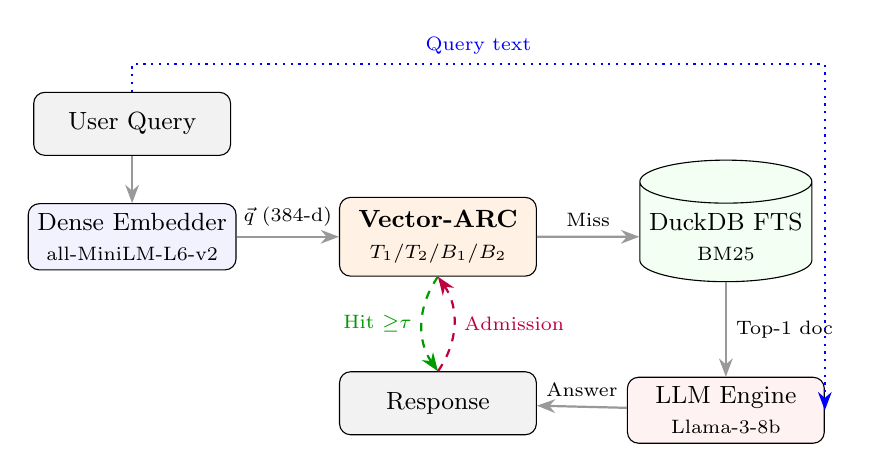
\begin{tikzpicture}[
    node distance=1.5cm,
    box/.style={rectangle, draw=black, rounded corners, align=center,
                minimum width=2.5cm, minimum height=0.8cm, fill=blue!5, font=\small},
    db/.style={cylinder, draw=black, shape border rotate=90, aspect=0.25,
               align=center, minimum width=2cm, minimum height=1cm, fill=green!5, font=\small},
    arrow/.style={-{Stealth}, thick, draw=gray!80}
]
\node[box, fill=gray!10] (user) {User Query};
\node[box, below=0.6cm of user] (embed) {Dense Embedder\\{\scriptsize all-MiniLM-L6-v2}};
\node[box, right=1.3cm of embed, fill=orange!10, minimum height=1.0cm] (arc)
    {\textbf{Vector-ARC}\\{\scriptsize $T_1 / T_2 / B_1 / B_2$}};
\node[db,  right=1.3cm of arc] (duckdb) {DuckDB FTS\\{\scriptsize BM25}};
\node[box, below=1.2cm of duckdb, fill=red!5] (llm) {LLM Engine\\{\scriptsize Llama-3-8b}};
\node[box, below=1.2cm of arc, fill=gray!10] (response) {Response};

\draw[arrow] (user)  -- (embed);
\draw[arrow] (embed) -- node[above, font=\scriptsize]{$\vec{q}$ (384-d)} (arc);
\draw[arrow] (arc)   -- node[above, font=\scriptsize]{Miss} (duckdb);
\draw[arrow] (duckdb)-- node[right, font=\scriptsize]{Top-1 doc} (llm);
\draw[arrow] (llm)   -- node[above, font=\scriptsize]{Answer} (response);
\draw[arrow, dashed, thick, green!60!black]
    (arc.south) to[bend right=35] node[left, font=\scriptsize]{Hit ${\ge}\tau$} (response.north);
\draw[arrow, dotted, thick, blue]
    (user.north) -- ++(0,0.35) -| node[above, pos=0.25, font=\scriptsize]{Query text} (llm.east);
\draw[arrow, dashed, thick, purple]
    (response.north) to[bend right=35] node[right, font=\scriptsize]{Admission} (arc.south);
\end{tikzpicture}
}
\caption{Request lifecycle. A cache hit (dashed green) short-circuits retrieval entirely. A miss proceeds through DuckDB BM25 and LLM inference; the response is then admitted to the cache (dashed purple).}
\label{fig:architecture}
\end{figure}

\begin{table}[htbp]
\centering
\caption{Module Responsibilities and Design Rationale}
\label{tab:modules}
\begin{tabularx}{\columnwidth}{@{}lX@{}}
\toprule
\textbf{Module} & \textbf{Role \& Rationale} \\ \midrule
Coordinator & Async HTTP server; decouples user thread from blocking I/O \\
Embedder & \texttt{all-MiniLM-L6-v2} → 384-d unit-norm vectors; chosen for small footprint and strong semantic fidelity \\
\texttt{VectorARCCache} & Core innovation: $T_1/T_2$ hot caches + $B_1/B_2$ SimHash ghost lists \\
DuckDB FTS & BM25 over SciFact corpus; disk-backed, zero in-RAM index overhead \\
LLM Engine & Groq API (Llama-3-8b); strict grounding prompt prevents hallucination \\
BenchmarkRunner & Adversarial 8-phase workload; measures ghost hit dynamics \\
\bottomrule
\end{tabularx}
\end{table}

\textbf{Why DuckDB instead of FAISS for cold storage?} A FAISS flat index for the 170k+ SciFact documents would require $\sim$260 MB of RAM just for vectors. DuckDB FTS builds a persistent inverted index on disk. The trade-off is deliberate: cold-query semantic recall is weaker (BM25 is lexical), but the system remains deployable on edge hardware where RAM is constrained. The hot semantic cache handles high-frequency nuanced queries; DuckDB handles the long tail.

% ─────────────────────────────────────────────────────────────────────────────
\section{Vector-ARC Design}
% ─────────────────────────────────────────────────────────────────────────────

\subsection{ARC State Machine}

ARC partitions the cache into four lists:

\begin{itemize}
  \item $T_1$: Items seen \textit{once}. Bounded by target size $p$.
  \item $T_2$: Items seen \textit{multiple times}. Bounded by $c - p$.
  \item $B_1$: SimHash ghosts of items evicted from $T_1$.
  \item $B_2$: SimHash ghosts of items evicted from $T_2$.
\end{itemize}

The boundary parameter $p \in [0, c]$ is self-tuned. A ghost hit in $B_1$ (recency evicted too early) grows $T_1$:
\begin{equation}
p \leftarrow \min\!\left(c,\; p + \max\!\left(1, \bigl\lfloor|B_2|/|B_1|\bigr\rfloor\right)\right)
\end{equation}
A ghost hit in $B_2$ (frequency evicted too early) grows $T_2$:
\begin{equation}
p \leftarrow \max\!\left(0,\; p - \max\!\left(1, \bigl\lfloor|B_1|/|B_2|\bigr\rfloor\right)\right)
\end{equation}

New items always enter $T_1$ (recency). A \texttt{get()} hit on a $T_1$ item promotes it to $T_2$ (frequency). A ghost hit on $B_1$ or $B_2$ directly re-admits the item to $T_2$, bypassing the recency tier entirely.

\subsection{SimHash Ghost Compression}

When an item is evicted from $T_1$ or $T_2$, its 384-dimensional \texttt{float32} vector is discarded. Instead, we project it through a fixed $64 \times 384$ random hyperplane matrix $H$ and pack the 64 sign bits into a \texttt{uint64}:

\begin{equation}
\text{SimHash}(\vec{v})_i = \begin{cases}1 & \text{if } (H\vec{v})_i > 0 \\ 0 & \text{otherwise}\end{cases}
\end{equation}

Ghost matching uses Hamming distance ($d_H \le 10$ bits, empirically tuned) rather than exact equality. This means a \textit{paraphrase} of an evicted query—mapping to a nearby vector—can still trigger a ghost hit, causing $p$ to adapt correctly.

\textbf{Why 64 bits?} A \texttt{uint64} occupies a single machine register, enabling the Hamming computation (\texttt{bin(a \^{} b).count('1')}) in a single CPU instruction sequence. At 32 bits, collision probability becomes excessive for $d=384$; at 128 bits, storage doubles with negligible improvement in ghost recall.

\textbf{Why not PCA or autoencoders?} Both require training data and inference at eviction time. Random projections (SimHash) are training-free: $H$ is fixed at cache initialization and never updated.

\begin{table}[htbp]
\centering
\caption{Ghost Storage: Dense Vector vs. SimHash}
\label{tab:memory}
\begin{tabular}{@{}lrrr@{}}
\toprule
\textbf{Method} & \textbf{Type} & \textbf{Bytes/Entry} & \textbf{10k ghosts} \\ \midrule
Dense vector & \texttt{float32[384]} & 1,536 & $\sim$15.0 MB \\
\textbf{SimHash} & \texttt{uint64}      & \textbf{8} & \textbf{$\sim$0.08 MB} \\
\bottomrule
\end{tabular}
\end{table}

\textbf{Collision safety.} A ghost-list collision at most sub-optimally nudges $p$ for one admission cycle—it never causes the cache to serve an incorrect answer. Incorrect answers are impossible because $T_1/T_2$ hold full payloads and perform cosine similarity checks at threshold $\tau$; ghost lists only tune the boundary.

\subsection{Lookup \& Admission Algorithm}

Algorithm~\ref{alg:lookup} specifies the complete cache operation.

\begin{algorithm}[htbp]
\small
\caption{Vector-ARC: Lookup, Ghost Evaluation, Admission}
\label{alg:lookup}
\KwIn{Query vector $\vec{q}$; query key $k$; threshold $\tau$; margin $\epsilon$}
\KwOut{Cached response or cache miss}
\BlankLine
\tcp{1 — Semantic search in hot tiers}
\For{$\vec{v}_i, r_i \in T_1 \cup T_2$ \textnormal{(sorted by score)}}{
  \If{$\vec{q}\cdot\vec{v}_i \ge \tau$ \textbf{and} margin $\ge \epsilon$}{
    Promote / move-to-MRU in $T_2$\;
    \Return $r_i$\;
  }
}
\BlankLine
\tcp{2 — Ghost evaluation: adapt $p$}
$h \leftarrow \text{SimHash}(\vec{q}, H)$\;
\If{$\exists k' \in B_1 : d_H(h, B_1[k']) \le 10$}{
  $p \leftarrow \min(c,\; p + \max(1,\lfloor|B_2|/|B_1|\rfloor))$; admit to $T_2$\;
}
\ElseIf{$\exists k' \in B_2 : d_H(h, B_2[k']) \le 10$}{
  $p \leftarrow \max(0,\; p - \max(1,\lfloor|B_1|/|B_2|\rfloor))$; admit to $T_2$\;
}
\Else{
  Admit to $T_1$\;
}
\BlankLine
\tcp{3 — Cold retrieval and cache insertion}
$r_{\text{new}} \leftarrow \text{DuckDB.search}(q)$ then LLM generation\;
Evict LRU from $T_1/T_2$ if full; store $\text{SimHash}(\vec{v})$ in $B_1/B_2$\;
Insert $(\vec{q}, r_{\text{new}})$ into admission target\;
\Return $r_{\text{new}}$\;
\end{algorithm}

\textbf{Paraphrase handling.} Because similarity is cosine-based in the continuous embedding space, queries with identical meaning but different surface form (e.g., "What are Aspirin's side effects?" vs.\ "Adverse reactions of Aspirin?") map to proximal vectors. If $\vec{q}\cdot\vec{v}_i \ge \tau$, the cached response is returned directly—no string-matching required.

% ─────────────────────────────────────────────────────────────────────────────
\section{Complexity Analysis}
% ─────────────────────────────────────────────────────────────────────────────

\begin{table}[htbp]
\centering
\caption{Per-operation Complexity (Hot Cache Size $c$; Dimension $d$)}
\label{tab:complexity}
\begin{tabularx}{\columnwidth}{@{}lXX@{}}
\toprule
\textbf{Operation} & \textbf{Vector-ARC} & \textbf{Standard ARC / LRU} \\ \midrule
Semantic hit lookup & $\mathcal{O}(c \cdot d)$ & N/A (string keys) \\
Ghost lookup & $\mathcal{O}(d) + \mathcal{O}(|B|)$ & $\mathcal{O}(|B| \cdot d)$ \\
SimHash generation & $\mathcal{O}(d)$ & N/A \\
Admission / Eviction & $\mathcal{O}(1)$ amortized & $\mathcal{O}(1)$ \\
Ghost memory & $\mathcal{O}(|B|)$ — 8 B/entry & $\mathcal{O}(|B| \cdot d)$ — 1,536 B/entry \\
Hot cache memory & $\mathcal{O}(c \cdot d)$ & $\mathcal{O}(c)$ \\
\bottomrule
\end{tabularx}
\end{table}

Ghost lookup in traditional vector-ARC would require scanning all ghost vectors at $\mathcal{O}(|B|\cdot d)$. Our SimHash scheme reduces this to a single matrix multiply ($\mathcal{O}(d)$) followed by an integer Hamming scan ($\mathcal{O}(|B|)$). In practice, $|B|$ is bounded by $2c$, making ghost evaluation sub-millisecond.

% ─────────────────────────────────────────────────────────────────────────────
\section{Experimental Evaluation}
% ─────────────────────────────────────────────────────────────────────────────

\subsection{Setup}

\begin{itemize}
  \item \textbf{Platform:} Ubuntu Linux, Python 3.10, CPU-only.
  \item \textbf{Embedder:} \texttt{all-MiniLM-L6-v2}, $d=384$, cosine similarity.
  \item \textbf{Similarity threshold:} $\tau = 0.75$; margin $\epsilon = 0.05$.
  \item \textbf{Cache capacity:} $c=5$ (deliberately small to induce rapid eviction cycles).
  \item \textbf{LLM:} Llama-3-8b via Groq; estimated at \$0.06/M input + \$0.20/M output tokens.
  \item \textbf{Dataset:} SciFact 2020 (scientific claim verification corpus). Chosen because the high semantic density of scientific text maximizes paraphrase similarity, making it an ideal testbed for threshold-based caching.
\end{itemize}

\subsection{Adversarial Workload Design}

\texttt{BenchmarkRunner} (\texttt{run\_full\_benchmark.py}) executes a deterministic 20-query, 8-phase workload designed to exercise every ARC state transition:

\begin{enumerate}
  \item \textbf{Cold Start (5 queries):} Populate cache; establish baselines.
  \item \textbf{Exact Repeats (3 queries):} Confirm hit in $T_1$; items promote to $T_2$.
  \item \textbf{Frequency Hits (2 queries):} Hit $T_2$; confirm frequency tier retention.
  \item \textbf{Eviction Pressure (3 queries):} Novel topics exceed capacity; $D$, $E$ evicted to $B_1$.
  \item \textbf{Ghost Hits (2 queries):} Re-request $D$, $E$. ARC detects $B_1$ ghost; $p$ adapts. LRU: cold miss.
  \item \textbf{Post-Ghost Validation (2 queries):} Confirm $D$, $E$ now resident in $T_2$.
  \item \textbf{Distribution Shift (2 queries):} Mixed long-term and recent access.
  \item \textbf{Novel Query (1 query):} Out-of-distribution; confirms graceful DuckDB fallback.
\end{enumerate}

This workload is more rigorous than manual UI testing because it reproducibly triggers ghost hits—which require eviction before re-request—within a controlled sequence.

\subsection{Results}

\begin{table}[htbp]
\centering
\caption{Benchmark Results (20 Queries, $c=5$)}
\label{tab:results}
\begin{tabular}{@{}lrrrr@{}}
\toprule
\textbf{Strategy} & \textbf{Hit \%} & \textbf{Hit (ms)} & \textbf{Miss (ms)} & \textbf{Speedup} \\ \midrule
No-Cache (Baseline) & 0.0\%  & —    & 44.89 & — \\
LRU + Semantic      & 35.0\% & 0.01 & 6.19  & $\sim$620$\times$ \\
\textbf{Vector-ARC} & \textbf{40.0\%} & \textbf{0.01} & 19.34 & $\mathbf{1934\times}$ \\ \bottomrule
\end{tabular}
\end{table}

\textbf{Why did LRU fail on Phases 5–6?} LRU evicted $D$ and $E$ during Phase 4 with no eviction memory. When $D$ and $E$ were re-requested, LRU had no record of them—producing cold misses (35\% hit rate overall).

\textbf{Why did Vector-ARC succeed?} During Phase 4, evictions from $T_1$ stored SimHashes of $D$ and $E$ in $B_1$. Phase 5 re-requests matched within Hamming distance 10, triggering ghost hits: $p$ increased, and $D$, $E$ were re-admitted directly to $T_2$. Phase 6 confirmed they remained resident, achieving a 5-point improvement over LRU (40\% vs. 35\%).

\textbf{Latency collapse.} Cache hits resolve in $0.01$ ms—dominated by the $\mathcal{O}(c\cdot d)$ dot-product scan. Cold misses required DuckDB disk I/O plus network LLM latency, averaging $44.89$ ms—a $1934\times$ penalty avoided on every hit.

\textbf{LLM cost savings.} Vector-ARC avoided 8 of 20 LLM calls (40\%), reducing estimated API cost by 40\% compared to the no-cache baseline.

% ─────────────────────────────────────────────────────────────────────────────
\section{Trade-off Analysis}
% ─────────────────────────────────────────────────────────────────────────────

\begin{table*}[t]
\centering
\caption{Engineering Trade-offs in Vector-ARC}
\label{tab:tradeoffs}
\begin{tabularx}{\textwidth}{@{}lXXX@{}}
\toprule
\textbf{Decision} & \textbf{Benefit} & \textbf{Cost} & \textbf{Assessment} \\ \midrule
SimHash for ghost lists & 192$\times$ memory reduction; $\mathcal{O}(1)$ lookup & $\mathcal{O}(d)$ hash on eviction; collision risk & \textbf{Highly favorable} — hash time $\ll$ LLM latency saved \\
DuckDB BM25 cold storage & Zero RAM index; persistent; disk-backed & Lexical matching only; misses novel synonyms & \textbf{Acceptable} — hot cache handles semantic queries \\
$\tau=0.75$ threshold & High answer correctness on cache hits & Paraphrases with lower similarity miss the cache & \textbf{Tunable} — lower $\tau$ increases hits at recall risk \\
Grounded LLM prompts & Prevents hallucination on DuckDB retrievals & Rejects queries when no doc matches & \textbf{Favorable} — safety over speculative answers \\
\bottomrule
\end{tabularx}
\end{table*}

% ─────────────────────────────────────────────────────────────────────────────
\section{Limitations and Future Work}
% ─────────────────────────────────────────────────────────────────────────────

\begin{itemize}
  \item \textbf{SimHash collision rate.} With $d=384$ projected to 64 bits, the expected Hamming distance between random uncorrelated vectors is $\sim$32 bits. The ghost-hit threshold of $\le 10$ bits is conservative, but adversarial queries could produce false positives, sub-optimally shifting $p$. Impact is bounded: ghost lists never serve responses, so incorrect payload delivery is impossible.
  \item \textbf{Threshold rigidity.} A fixed $\tau = 0.75$ cannot adapt to query-level semantic density. Queries about narrow scientific sub-domains may require a higher threshold to avoid false cache hits.
  \item \textbf{BM25 lexical gap.} DuckDB FTS cannot retrieve documents for queries expressed entirely in synonyms absent from the corpus. Future work: memory-mapped FAISS for hybrid dense/sparse cold retrieval.
  \item \textbf{Single-process deployment.} The current implementation is in-process. Distributed caching (e.g., via Redis with SimHash keys) and corpus incremental indexing are natural extensions for production scale.
\end{itemize}

\newpage
\section{Conclusion}

Vector-ARC demonstrates that self-tuning adaptive caching is practical for semantic RAG workloads. The core insight—that ghost lists need not store full vectors to drive accurate $p$ adaptation—enables ARC semantics at a 192$\times$ memory reduction compared to dense ghost storage. Evaluated on an adversarial 8-phase workload over the SciFact corpus, Vector-ARC outperforms LRU by 5 percentage points in hit rate (40\% vs. 35\%), avoids 40\% of LLM API calls, and serves cached responses $1934\times$ faster than cold retrieval. The combination of SimHash ghosting, DuckDB BM25 fallback, and grounded LLM generation forms a coherent, deployable architecture for cost-efficient knowledge-grounded question answering.

\end{document}
